\documentclass[discrete.tex]{subfiles}

\begin{document}
  \section{Приближенные методы решения дискретных задач}
  NP - класс всех задач поиска

  P - класс всех задач поиска, решение которых может быть найдено за полиноминальное время

  $P \neq NP$ - нерешенная задача

  Задача поиска называется NP-полной, если к ней сводятся все залачи посика. В предположении $P \neq NP$ не существует полиноминальных точных алгоритмов для NP-полных задач. Для них можно найти в течении полиноминального времени решение, близкое к оптимальному. Алгоритм, возвращающий такие решения называется приближенным
  \begin{figure}[H]
      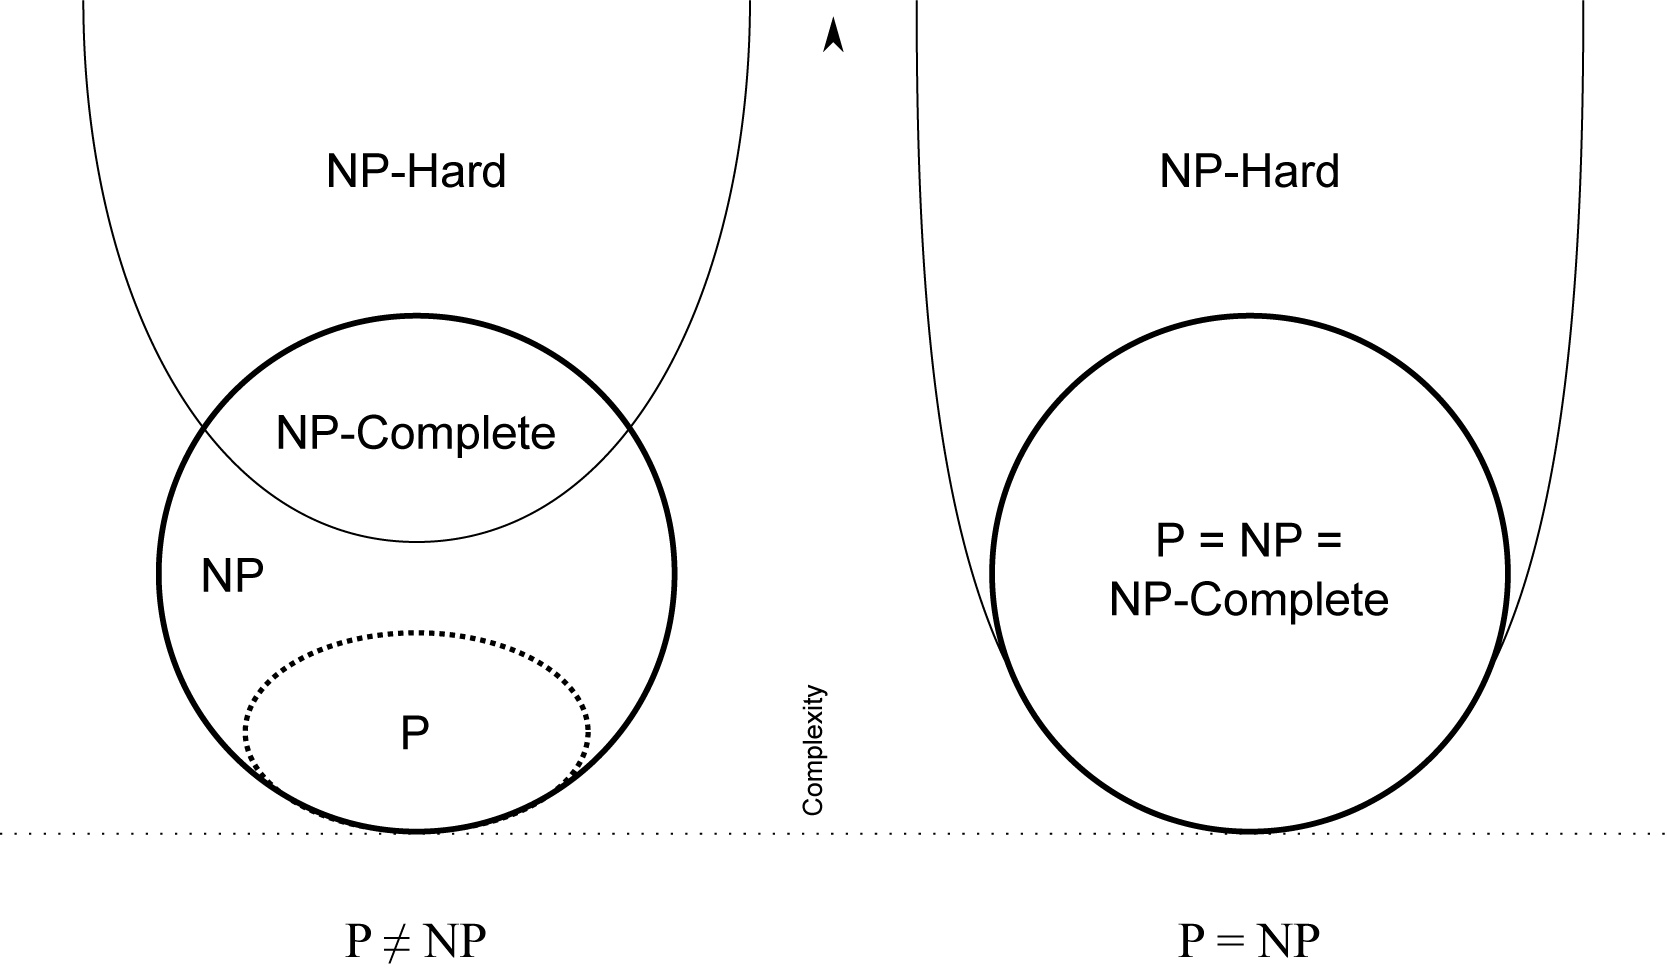
\includegraphics[width=10cm]{pics/58_1.png}
      \centering
  \end{figure}

  \begin{example}[приближенные алгоритмы]
    \begin{enumerate}
      \item Жадные алгоритмы
      \item Алгоритмы с гарантированной оценкой точности
      \item $\E$-приближенные алгоритмы
      \item Локальный поиск
      \item Генетические алгоритмы
      \item Муравьиные алгоритмы
      \item Нейронные сети
      \item Гибридные алгоритмы
    \end{enumerate}

    \begin{enumerate}
      \item Жадный алгоритм на каждом шаге делает локально наилучший выбор в надежде, что итоговое решение будет оптимальным (Алгоритм Дейкстры, задача о рюкзаке не всегда подходит, Алгорим Краскала)

      Жадный алгоритм не всегда дает наилучший результат
      \item Точность приближенного алгоритма измеряется в том, в какое максимальное число раз может отличаться полученное решение от оптимального :
      \[\e k: \frac{f_a}{f_{opt}} \leq k \text{ - гарантированная оценка точности}\]
      Алгоритм Кристофидеса $k=2$, алг. К. с оценкой $\frac{3}{2}$
      \item $\E$-прибл. алг., если $\forall \E>0$ можно построить алг.:
      \[\frac{f_a - f_{opt}}{f_{opt}} < E\]
      \item Локальный поиск - поиск, который учитывает текущее состояние, а ранее пройденные не учитываются. Основная задача - не нахождение оптимального пути к целевой точки, а оптимизация некоторой целевой функции
      \item Генетический алгоритм - эвристический алгоритм поиска. Описание:
      \begin{enumerate}
        \item Задаит целевую функцию для особой популяции
        \item Создать начальную популяцию *начало цикла*:
        \begin{enumerate}
          \item Размножение
          \item Мутирование
          \item Целевая функция для всех особоей
          \item Формирование нового поколения
          \item Если выполнятся условия остановки цикла, конец
        \end{enumerate}
      \end{enumerate}
      Когда остановились - нашли решение
      \item Муравьиный алгорим (один из алгоритмов решения задачи коммивояжера). В вершинах графа (городах) размещаем муравьев. Начинается их движение, направление определяется вероятностными методами (*маркировка наиболее удачных путей*)
      \item Нейронная сеть - математическая модель, система соединенных и взаимод. между собой процессов. Обучается (нахождение коэф. связей между нейронами)
      \item Гибридные алгоритмы - сочетают разные подходы
    \end{enumerate}
  \end{example}

\end{document}
